\documentclass{standalone}

%%%%%%%%%%%%%%%%%%%%%%%%%%%%%%%%%%%%%%
% Packages ---------------------------------------------------------
%%%%%%%%%%%%%%%%%%%%%%%%%%%%%%%%%%%%%%
\usepackage[version=4]{mhchem}				 % chemical reactions environment
\usepackage{tikz}										 % Tikz package
\usetikzlibrary{arrows.meta}						% Pacakge for Arrows
\usepackage{amssymb} 								% Package for empty set

%%%%%%%%%%%%%%%%%%%%%%%%%%%%%%%%%%%%%%
% Commands  ------------------------------------------------------
%%%%%%%%%%%%%%%%%%%%%%%%%%%%%%%%%%%%%%
\renewcommand{\familydefault}{\sfdefault}        	% Change Font
\let\emptyset\varnothing

%%%%%%%%%%%%%%%%%%%%%%%%%%%%%%%%%%%%%%
% Commands  ------------------------------------------------------
%%%%%%%%%%%%%%%%%%%%%%%%%%%%%%%%%%%%%% 
\newcommand{\species}[1]{{\bf\ce{#1}}}
\newcommand{\UP}[1]{\makebox[0pt]{\smash{\raisebox{1em}{\normalsize #1}}}}
\newcommand{\RT}[1]{\makebox[0pt]{\hspace{5em}$#1$}}

%%%%%%%%%%%%%%%%%%%%%%%%%%%%%%%%%%%%%%
% Colors ------------------------------------------------------------
%%%%%%%%%%%%%%%%%%%%%%%%%%%%%%%%%%%%%%
\definecolor{Repressor}{RGB}{228,26,28}
\definecolor{Activator}{RGB}{77,175,74}
\definecolor{NAR}{RGB}{150,150, 150}

%%%%%%%%%%%%%%%%%%%%%%%%%%%%%%%%%%%%%%
% Elements  --------------------------------------------------------
%%%%%%%%%%%%%%%%%%%%%%%%%%%%%%%%%%%%%%
\newcommand{\Species}[5]{ % Inputs: coordinates, scale, color, name, textcolor
	\begin{scope}[shift = {(#1)}, scale = #2]	
		\filldraw[fill=#3, draw=black, thick] (0,0) circle (0.5cm);
		%		\filldraw[fill=#3, draw=black, thick, blur shadow ={shadow opacity=80, shadow blur steps=50}] (0,0) circle (0.5cm);
		\node[anchor = center, #5] at (0,0) {\Large #4};
	\end{scope}
}

\newcommand{\Dimer}[6]{ % Inputs: coordinates, scale, color, name, textcolor, rotation
	\begin{scope}[shift = {(#1)}, scale = #2, rotate = #6]	
		\filldraw[fill=#3, draw=black, thick] (0.3,0) circle (0.5cm);
		\filldraw[fill=#3, draw=black, thick] (-0.3,0) circle (0.5cm);
		\filldraw[fill=#3, draw = #3] (-0.3,-0.38) rectangle (0.3,0.28);
		\node[anchor = center, #5] at (0,0) {\Large #4};
	\end{scope}
}

\newcommand{\Trimer}[6]{ % Inputs: coordinates, scale, color, name, textcolor, rotation
	\begin{scope}[shift = {(#1)}, scale = #2, rotate = #6]	
		\filldraw[fill=#3, draw=black, thick] (0,0) circle (0.5cm);
		\filldraw[fill=#3, draw=black, thick] (0.65,0) circle (0.5cm);
		\filldraw[fill=#3, draw=black, thick] (-0.65,0) circle (0.5cm);
		\filldraw[fill=#3, draw = #3] (-0.3,-0.35) rectangle (0.3,0.28);
		\node[anchor = center, #5] at (0,0) {\Large #4};
	\end{scope}
}

\newcommand{\SingleCharge}[4]{ % Inputs: coordinates, scale, rotation, Charge
	\begin{scope}[shift = {(#1)}, scale = #2, rotate = #3]	
		\filldraw[fill=yellow!50, draw=black, ultra thick, rounded corners = 0.1] (-0.2,-0.2) rectangle(0.2,0.2);
		\node [anchor = center] at (0,0) {\Large #4};
	\end{scope}
}

\newcommand{\DoubleCharge}[5]{ % Inputs: coordinates, scale, rotation, Charge1, Charge2
	\begin{scope}[shift = {(#1)}, scale = #2, rotate = #3]	
		\filldraw[fill=yellow!50, draw=black, ultra thick, rounded corners = 0.1] (-0.4,-0.2) rectangle(0,0.2);
		\filldraw[fill=yellow!50, draw=black, ultra thick, rounded corners = 0.1] (0,-0.2) rectangle(0.4,0.2);
		\node [anchor = center] at (-0.2,0) {\Large #4};
		\node [anchor = center] at (0.2,0) {\Large #5};
	\end{scope}
}

\newcommand{\TripleCharge}[6]{ % Inputs: coordinates, scale, rotation, Charge1, Charge2, Charge3
	\begin{scope}[shift = {(#1)}, scale = #2, rotate = #3]	
		\filldraw[fill=yellow!50, draw=black, ultra thick, rounded corners = 0.1] (-0.6,-0.2) rectangle(-0.2,0.2);
		\filldraw[fill=yellow!50, draw=black, ultra thick, rounded corners = 0.1] (-0.2,-0.2) rectangle(0.2,0.2);
		\filldraw[fill=yellow!50, draw=black, ultra thick, rounded corners = 0.1] (0.2,-0.2) rectangle(0.6,0.2);
		\node [anchor = center] at (-0.4,0) {\Large #4};
		\node [anchor = center] at (0,0) {\Large #5};
		\node [anchor = center] at (0.4,0) {\Large #6};
	\end{scope}
}
%%%%%%%%%%%%%%%%%%%%%%%%%%%%%%%%%%%%%%
% Documents Begins Here ------------------------------------------
%%%%%%%%%%%%%%%%%%%%%%%%%%%%%%%%%%%%%%
\begin{document}
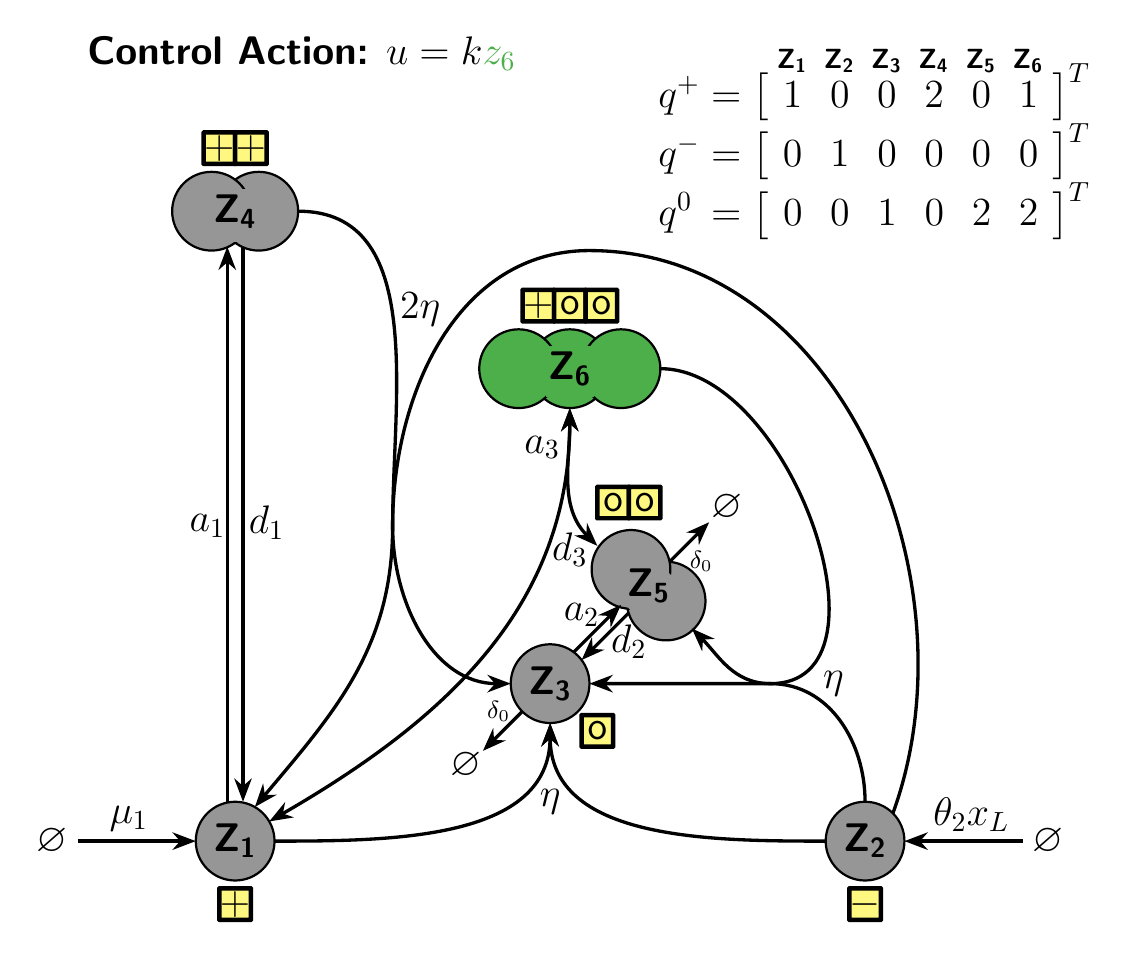
\begin{tikzpicture} 
%\draw [step=1, very thin, orange] (-8,-1) grid (8,10); 
%%%%%%%%%%%%%%%%%%%%%%%%%%%%%%%%%%%%%%
% Blocks -----------------------------------------------------------
%%%%%%%%%%%%%%%%%%%%%%%%%%%%%%%%%%%%%%
%\filldraw [IColor!15, rounded corners = 10] (-6.7,-3.2) rectangle (9,0.6);
				
%%%%%%%%%%%%%%%%%%%%%%%%%%%%%%%%%%%%%%
% Species -----------------------------------------------------------
%%%%%%%%%%%%%%%%%%%%%%%%%%%%%%%%%%%%%%
\Species{(-4,0)}{1}{NAR}{\species{Z_1}}{black};
\Species{(4,0)}{1}{NAR}{\species{Z_2}}{black};
\Species{(0,2)}{1}{NAR}{\species{Z_3}}{black};
\Dimer{(-4,8)}{1}{NAR}{\species{Z_4}}{}{0};
\Dimer{(1.25,3.25)}{1}{NAR}{\species{Z_5}}{black}{-42};
\Trimer{(0.25,6)}{1}{Activator}{\species{Z_6}}{black}{0};

%%%%%%%%%%%%%%%%%%%%%%%%%%%%%%%%%%%%%%
% Charges ----------------------------------------------------------
%%%%%%%%%%%%%%%%%%%%%%%%%%%%%%%%%%%%%%
\SingleCharge{(-4,-0.8)}{1}{0}{$+$}; % Z1
\SingleCharge{(4,-0.8)}{1}{0}{$-$}; % Z2
\SingleCharge{(0.6,1.4)}{1}{0}{o}; % Z3
\DoubleCharge{(1,4.3)}{1}{0}{o}{o}; % Z4
\DoubleCharge{(-4,8.8)}{1}{0}{$+$}{$+$}; % Z5
\TripleCharge{(0.25,6.8)}{1}{0}{$+$}{o}{o}; % Z6

%%%%%%%%%%%%%%%%%%%%%%%%%%%%%%%%%%%%%%
% Arrows -----------------------------------------------------------
%%%%%%%%%%%%%%%%%%%%%%%%%%%%%%%%%%%%%%
\draw [->, -Stealth, very thick] (-6,0) -- (-4.5,0); % Production of Z1
\draw [->, -Stealth, very thick] (6,0) -- (4.5,0); % Production of Z2
\draw [->, -Stealth, very thick] (-3.5, 0) to [out = 0, in = -90] (0,1.5); % Sequestration of Z1 with Z2
\draw [->, -Stealth, very thick] (3.5, 0) to [out = 180, in = -90] (0,1.5); % Sequestration of Z2 with Z1
\draw [->, -Stealth, very thick] (0.3,2.4) -- (0.9,3); % Association of Z3
\draw [->, -Stealth, very thick] (1,2.9) -- (0.4,2.3); % Dissociation of Z4
\draw [->, -Stealth, very thick] (-4.1,0.5) -- (-4.1,7.55); % Association of Z1
\draw [->, -Stealth, very thick] (-3.9,7.55) -- (-3.9,0.5); % Dissociation of Z5
\draw [->, -Stealth, very thick] (1.4, 6) to [out = 0 , in = 0] (2.8,2) to [out =180 , in = -45] (1.8, 2.7); % Production of Z4 from Z2-Z6 Sequestration
\draw [->, -Stealth, very thick] (4, 0.5) to [out = 90 , in = 0] (2.8,2) -- (0.5,2); % Production of Z3 from Z2-Z6 Sequestration
\draw [->, -Stealth, very thick] (4.3536, 0.3536) to [out = 70, in = 0] (0.5,7.5) to [out =180 , in = 90] (-2,4) to [out = -90, in = 180] (-0.5,2); % Production of Z3 from Z2-Z5 Sequestration
\draw [->, -Stealth, very thick] (-3.2,8) to [out = 0, in = 90 ] (-2,4) to [out = -90, in = 50] (-4 + 0.5*cos{60}, 0.5*sin{60}); % Production of Z1 from Z2-Z5 Sequestration
\draw [>=Stealth,  <->, very thick] (0.6,3.75) to [out = 90+45, in = -90] (0.25,5.5); % Association of Z6 from Z4
\draw [>=Stealth,  <->, very thick] (-4+0.5*cos{30},0.5*sin{30}) to [out = 30, in = -90] (0.25,5.5); % Association of Z6 from Z1
\draw [->, -Stealth, very thick] (0 - 0.5*cos{45}, 2 - 0.5*sin{45}) -- (0 - 0.5*cos{45}-0.5, 2 - 0.5*sin{45}-0.5); % Degradation of Z3
\draw [->, -Stealth, very thick] (1.25  +0.27, 3.25 + 0.3) -- (1.25 +0.27+0.5, 3.25 +0.3 + 0.5); % Degradation of Z5

%%%%%%%%%%%%%%%%%%%%%%%%%%%%%%%%%%%%%%
% Empty Sets -------------------------------------------------------
%%%%%%%%%%%%%%%%%%%%%%%%%%%%%%%%%%%%%%
\node [anchor = east] at (-6,0) {\Large $\emptyset$}; % Production of Z1
\node [anchor = west] at (6,0) {\Large $\emptyset$}; % Production of Z2
\node [anchor = north east] at ((0 - 0.5*cos{45}-0.5+0.1, 2 - 0.5*sin{45}-0.5+0.1) {\Large $\emptyset$}; % Degradation of Z3
\node [anchor = south west] at (1.25 +0.27+0.5 - 0.1, 3.25 +0.3 + 0.5 - 0.1) {\Large $\emptyset$}; % Degradation of Z5

%%%%%%%%%%%%%%%%%%%%%%%%%%%%%%%%%%%%%%
% Rates -------------------------------------------------------------
%%%%%%%%%%%%%%%%%%%%%%%%%%%%%%%%%%%%%%
\node [anchor = south] at (-5.35,0) {\Large $\mu_1$}; % Production of Z1
\node [anchor = south] at (5.35,0) {\Large $\theta_2 x_L$}; % Production of Z2
\node [anchor = center] at (0,0.5) {\Large $\eta$}; % Sequestration of Z1 and Z2
\node [anchor = center] at (-1.65,6.75) {\Large $2\eta$}; % Sequestration of Z5 and Z2
\node [anchor = center] at (3.6,2) {\Large $\eta$}; % Sequestration of Z6 and Z2
\node [anchor = east] at (-4,4) {\Large $a_1$}; 
\node [anchor = west] at (-3.95,4.05) {\Large $d_1$}; 
\node [anchor = east] at (0.25,5) {\Large $a_3$}; 
\node [anchor = center] at (0.25,3.7) {\Large $d_3$}; 
\node [anchor = south] at (0.4,2.6) {\Large $a_2$}; 
\node [anchor = south] at (1,2.2) {\Large $d_2$}; 
\node [anchor = center] at ((0 - 0.5*cos{45}-0.3, 2 - 0.5*sin{45}) {\small $\delta_0$};
\node [anchor = center] at (1.25 +0.27+0.5 - 0.1, 3.25 +0.3 ) {\small $\delta_0$};

%%%%%%%%%%%%%%%%%%%%%%%%%%%%%%%%%%%%%%
% Labels ------------------------------------------------------------
%%%%%%%%%%%%%%%%%%%%%%%%%%%%%%%%%%%%%%
\node [anchor = west] at (-6,10) {\Large \textbf{Control Action:} $u = k\textcolor{Activator}{z_6}$};
\node [anchor = west] at (1.25,9.5) {\Large $q^+ = \left[ \arraycolsep=5pt
																				\begin{array}{cccccc} 
																					\UP{~~\species{Z_1}}{1} & \UP{~~\species{Z_2}}{0} & \UP{~~\species{Z_3}}{0} & \UP{~~\species{Z_4}}{2}& \UP{~~\species{Z_5}}{0}& \UP{~~\species{Z_6}}{1}
																				\end{array}\right]^T$};
\node [anchor = west] at (1.25,8.75) {\Large $q^- = \left[ \arraycolsep=5pt
																				\begin{array}{cccccc} 
																					\UP{}{0} & \UP{}{1} & \UP{}{0} & \UP{}{0}& \UP{}{0}& \UP{}{0}
																				\end{array}\right]^T$};		
\node [anchor = west] at (1.25,8) {\Large $q^{0\hspace{0.1cm}} = \left[ \arraycolsep=5pt
																				\begin{array}{cccccc} 
																					\UP{}{0} & \UP{}{0} & \UP{}{1} & \UP{}{0}& \UP{}{2}& \UP{}{2}
																				\end{array}\right]^T$};			
%\node [anchor = north] at (0,-0.5) {\Large \ce{\species{Z_i} ->[$\delta$] $\emptyset$}};																
\end{tikzpicture}
	
%%%%%%%%%%%%%%%%%%%%%%%%%%%%%%%%%%%%%%
% Documents Ends Here ------------------------------------------------
%%%%%%%%%%%%%%%%%%%%%%%%%%%%%%%%%%%%%%
\end{document}  